\chapter{Propriedades das Séries de Fourier}
\section{Teorema de Parseval}
\begin{defn} 
Define-se a potência média de um função periódica $f(t)$ como
\begin{equation}\overline{P}_f=\frac{1}{T}\int_0^T |f(t)|^2dt\end{equation}
\end{defn}
\begin{ex}{\label{ex_1_cap_5}} A potência média da função $f(t)=A\cos(wt)$ é dada por
\begin{eqnarray*}
\overline{P}_f&=&\frac{1}{T}\int_0^T |f(t)|^2dt\\
&=&\frac{1}{T}\int_0^{T} A^2\cos\left(\frac{2\pi}{T} t\right)^2dt\\
&=&\frac{A^2}{T}\int_0^{T} \left(\frac{\cos\left(\frac{4\pi}{T} t\right)+1}{2}  \right)dt\\
&=&\frac{A^2}{2}
\end{eqnarray*}
 onde se usou que $w=\frac{2\pi}{T}$ e identidade trigonométrica dada por:
\begin{equation}\cos^2(x)=\left(\frac{e^{ix}+e^{-ix}}{2}\right)^2=\frac{e^{2ix}+2+e^{-2ix}}{4}=\frac{\cos(2x)+1}{2}.\end{equation}
 \end{ex}
\begin{ex} Seja $V(t)=A\cos(wt)$ uma fonte de tensão com frequência $w=60$\ \!\!Hz $=120\pi$\ \!\!rad/s ligado a um resistor de resitência $R\Omega$. A potência no resistor é
\begin{equation}
P(t)=\frac{V(t)^2}{R}
\end{equation}
e a potência média $P_m$ é
\begin{equation}
P_m=\frac{1}{T}\int_0^TP(t)dt=\frac{1}{T}\int_0^T\frac{V(t)^2}{R}dt,
\end{equation}
onde $T=\frac{1}{60}s$. Por outro lado, a potência média é calculada em termos da tensão média por
\begin{equation}
P_m=\frac{V_m^2}{R},
\end{equation}
ou seja,
\begin{equation}{\label{valor_RMS}}
V_m^2=\frac{1}{T}\int_0^T V(t)^2 dt.
\end{equation}
O exemplo \ref{ex_1_cap_5} nos dá o valor da potência média do sinal $V(t)=A\cos(wt)$. Logo,
\begin{equation}
V_m=\frac{A}{\sqrt{2}}.
\end{equation}
Se $V_m=127V$, então a amplitude do sinal é aproximadamente $A\approx 180$.
\end{ex}
\begin{obs}Na expressão (\ref{valor_RMS}), $V_m$ também é chamado de valor RMS do sinal $v(t)$ (Root mean square):
\begin{equation}
V_{RMS}=\sqrt{\frac{1}{T}\int_0^T V(t)^2 dt}.
\end{equation}
\end{obs}
\begin{teo}[Teorema de Parseval] Seja $f(t)$ uma função periódica representável por uma série de Fourier, então vale a seguinte identidade.
\begin{equation}\label{teo_parseval} 
\frac{1}{T}\int_0^T |f(t)|^2dt=\sum_{n=-\infty}^\infty |C_n|^2.
 \end{equation}
\end{teo}
\begin{proof}
\begin{eqnarray*}
 \frac{1}{T}\int_0^T |f(t)|^2dt&=&\frac{1}{T}\int_0^T f(t)\overline{f(t)}dt
\end{eqnarray*}
 Como $\displaystyle f(t)=\sum_{n=-\infty}^\infty C_n e^{iw_n t}$, temos
 \begin{eqnarray*}
  \overline{f(t)}&=&\overline{\sum_{n=-\infty}^\infty C_n e^{iw_n t}}
  =\sum_{n=-\infty}^\infty \overline{C_n}~ \overline{e^{iw_n t}}
  =\sum_{n=-\infty}^\infty \overline{C_n} e^{-iw_n t}
 \end{eqnarray*}
Substituindo esta expressão para $\overline{f(t)}$ na definição de potência média, temos:
\begin{eqnarray*}
 \frac{1}{T}\int_0^T |f(t)|^2dt&=&\frac{1}{T}\int_0^T f(t)\overline{f(t)}dt=\frac{1}{T}\int_0^Tf(t)\left[\sum_{n=-\infty}^\infty \overline{C_n} e^{-iw_n t}\right] dt\\
 &=&\frac{1}{T}\sum_{n=-\infty}^\infty\left[\overline{C_n}\int_0^Tf(t)e^{-iw_nt}dt\right]
 \end{eqnarray*}
 Como $C_n=\frac{1}{T}\int_0^Tf(t)e^{-iw_nt}dt$, temos:
\begin{eqnarray*}
 \frac{1}{T}\int_0^T |f(t)|^2dt&=&\sum_{n=-\infty}^\infty\overline{C_n}C_n = \sum_{n=-\infty}^\infty|C_n|^2
 \end{eqnarray*}
\end{proof}
\begin{ex}\label{ex_quadrada_parseval} Seja $g(t)$ um função dada no exemplo \ref{ex_quadrada}, isto é,
\begin{eqnarray*}
g(t)&=&-1, \ \ -1< t<0\\
g(t)&=&0, \ \ t=0\ \hbox{ou}\ t=1\\
g(t)&=&1, \ \ 0< t<1\\
g(t+2)&=&g(t),\ \ \forall t\in\mathbb{R}.
\end{eqnarray*}
\begin{figure}[!ht]
\begin{center}
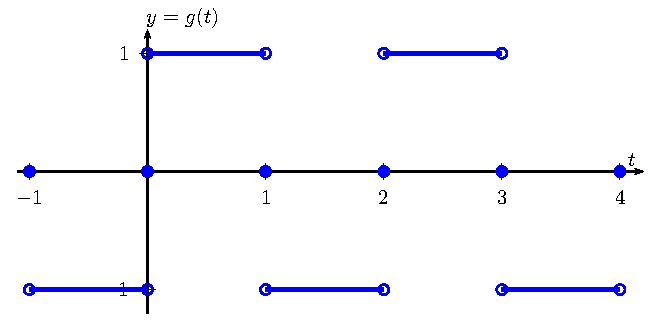
\includegraphics{cap_propriedades_series/pics/figura_1}\end{center}
\end{figure}
Vimos no exemplo \ref{ex_quadrada} que sua expansão em série de Fourie é da forma:
\begin{equation}
g(t)=\frac{4}{\pi}\left(\sen(\pi t)+\frac{1}{3}\sen(3\pi t)+\frac{1}{5}\sen(5\pi t)+\cdots\right).
\end{equation}
Calcularemos agora a potência média desta função através de sua representação no tempo e depois em frequência:
\begin{eqnarray*}
 \overline{P_f}=\frac{1}{T}\int_0^T |g(t)|^2dt=\frac{1}{2}\int_0^2 |g(t)|^2dt=\frac{1}{2}\int_0^2 1dt=1
\end{eqnarray*}
Alternativamente, temos pelo Teorema de Parseval:
\begin{eqnarray*}
 \overline{P_f}=\sum_{n=-\infty}^\infty |C_n|^2=\sum_{n=-\infty}^\infty \left|\frac{a_n-ib_n}{2}\right|^2=\frac{1}{4}\sum_{n=-\infty}^\infty |b_n|^2
\end{eqnarray*}
Como $b_{-n}=b_n$, temos que $|b_{-n}|=|b_n|$ e ainda temos que $b_0=0$, portanto: 
\begin{eqnarray*}
 \overline{P_f}=\frac{1}{2}\sum_{n=1}^\infty |b_n|^2 = \frac{1}{2}\left(\frac{4}{\pi}\right)^2\left(1 + \frac{1}{3^2}+ \frac{1}{5^2}+ \frac{1}{7^2}+\cdots\right)
\end{eqnarray*}
usando a equação (\ref{serie_inv_impar}) da página \pageref{serie_inv_impar}, temos:
\begin{eqnarray*}
 \overline{P_f}=\frac{1}{2}\left(\frac{4}{\pi}\right)^2\frac{\pi^2}{8}=1
\end{eqnarray*}
\end{ex}

\subsection*{Exercícios}
\begin{exer}Dado o diagrama de espectro de amplitude de uma função periódica $f(t)$, marque as alternativas que representam, respectivamente, o módulo do valor médio e a potência média da função $\left(\left|\frac{1}{T}\int_0^Tf(t)dt\right|\quad\text{e}\quad \frac{1}{T}\int_0^T|f(t)|^2dt\right)$.
\begin{figure}[!ht]
\begin{center}
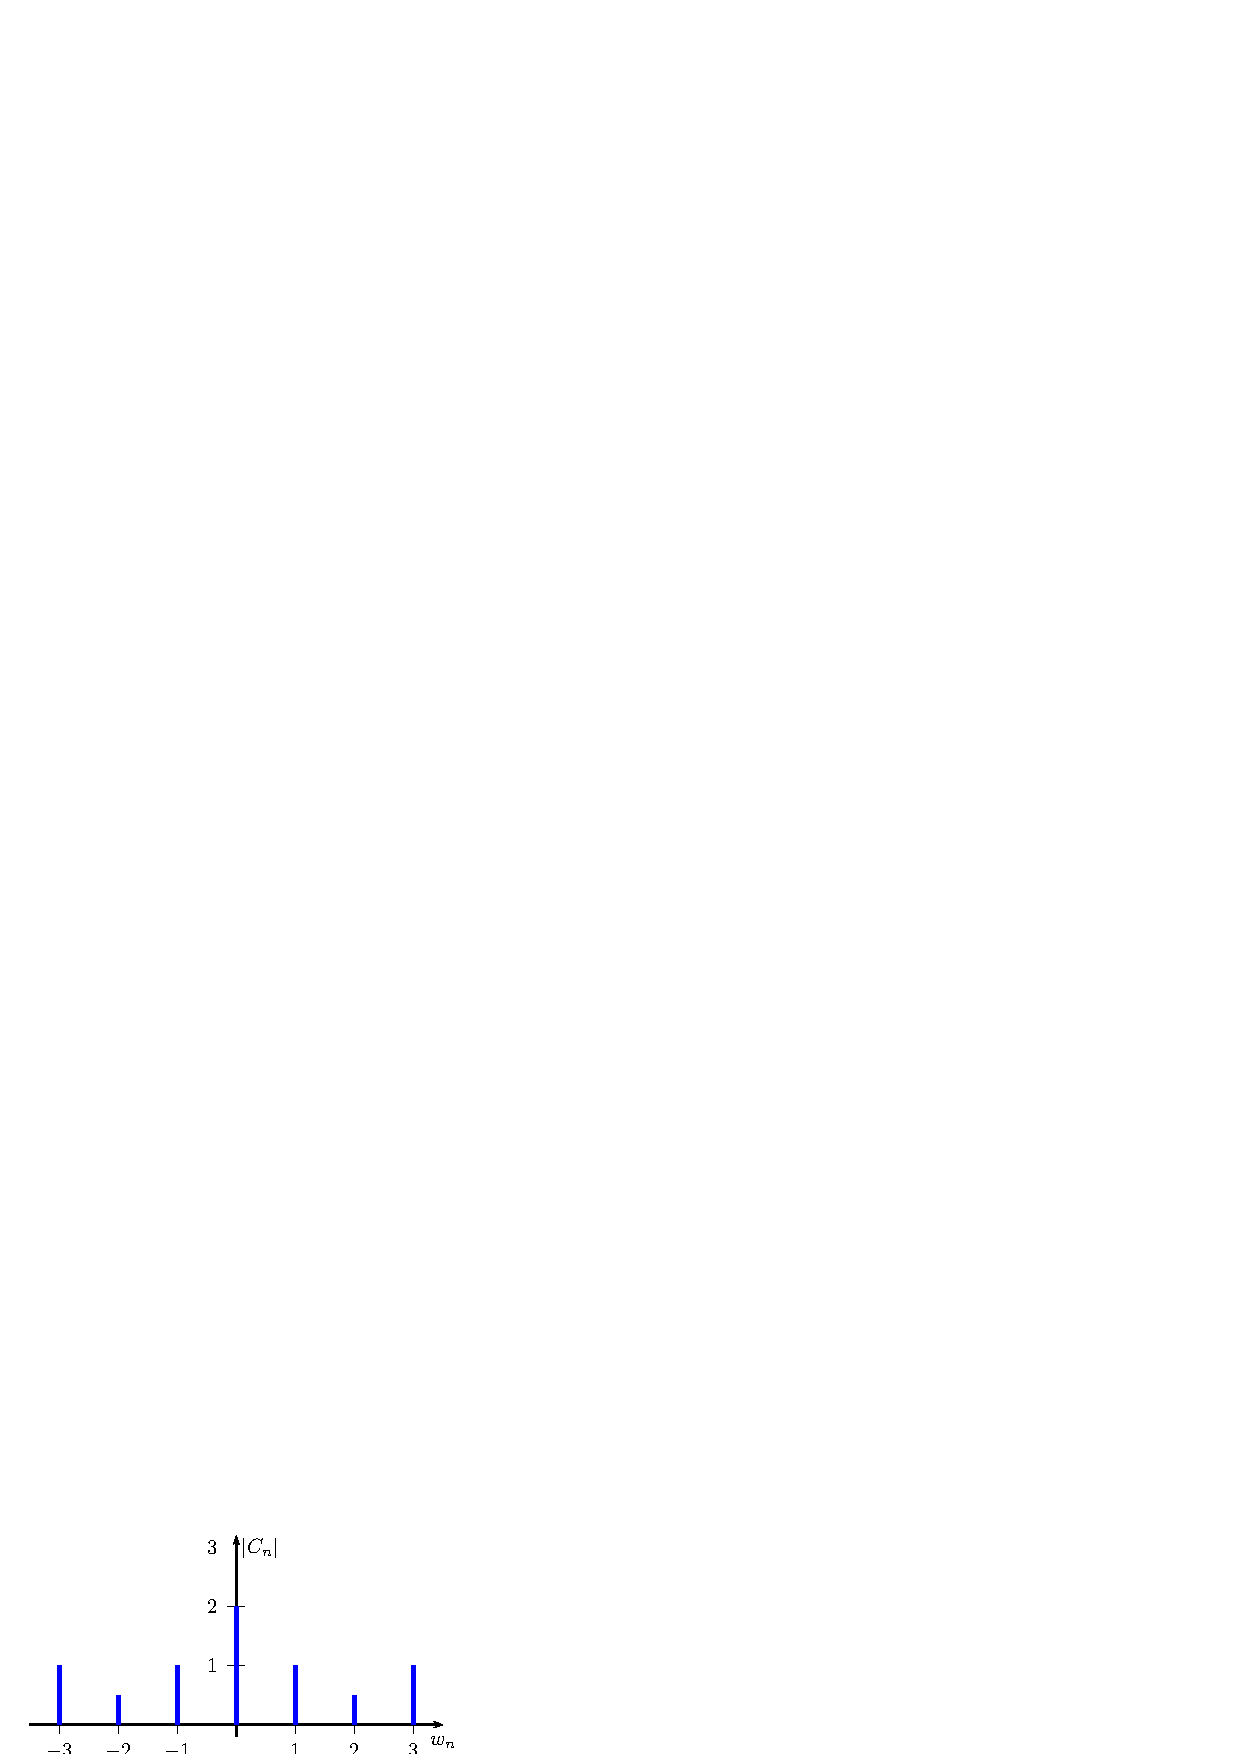
\includegraphics{cap_propriedades_series/pics/figura_4}\end{center}
\end{figure}

\begin{minipage}{8cm}
{Valor Médio}
 \begin{itemize}
 \item[(\ \ )] 0
 \item[(\ \ )] 0.5
 \item[(\ \ )] 1
 \item[(\ \ )] 1.5
 \item[(\ \ )] 2 %esta
 \item[(\ \ )] 2.5
 \item[(\ \ )] 3
 \end{itemize}
\end{minipage}
\begin{minipage}{8cm}
{Potência Média}
 \begin{itemize}
\item[(\ \ )]  11.5
 \item[(\ \ )] 10
 \item[(\ \ )] 8.5 %esta
 \item[(\ \ )] 6
 \item[(\ \ )] 4.5
 \item[(\ \ )] 3
 \item[(\ \ )] 0.5
 \end{itemize}
\end{minipage}
\end{exer}
\section{Fenômeno de Gibbs}
A convergência das somas parciais da série de Fourier de uma função suave por partes em torno de um salto apresenta oscilações cujas amplitudes não convergem para zero. A convergência ponto a ponto acontece, mas se olharmos para o valor absoluto da diferença entre a função e soma parcial sempre encontramos um ponto onde esse valor é aproximadamente 8,9\% da amplitude do salto. Esse fenômeno é chamado de Fenômeno de Gibbs
\begin{figure}[!ht]
\begin{center}
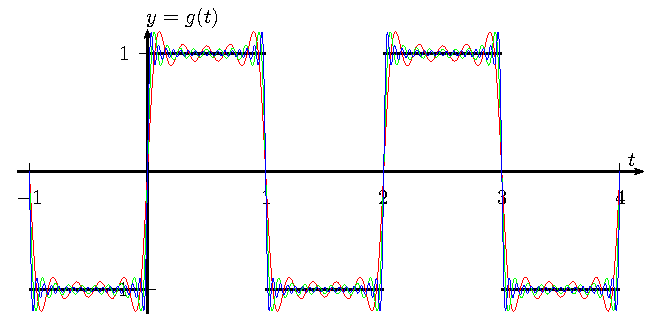
\includegraphics{cap_propriedades_series/pics/figura_2}\end{center}
\end{figure}
\begin{figure}[!ht]
\begin{center}
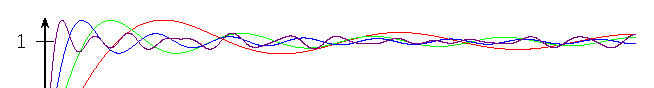
\includegraphics{cap_propriedades_series/pics/figura_3}\end{center}
\end{figure}
